%!TEX root = ./jctt.tex

\section{Computational Results}


We first consider a test problem that is homogeneous with a reflecting left boundary, vacuum right boundary, and a total thickness of \SI{10}{cm}.  The total and scattering macroscopic cross sections were set to \SI{1}{cm^{-1}} and 
\SI{0.99}{cm^{-1}} leading to a scattering ratio of $c = \frac{\sigma_s}{\sigma_t}=0.99$. With 50 spatial cells the optical thickness per cell was 0.2 mfp and the domain thickness was 10 mfp. The isotropic fixed source was set to \SI{1}{\particles\per\second\per\cm\cubed}. 
Unless otherwise indicated in this section, all calculations were performed with 50 uniform spatial cells and S$_8$ Gauss quadrature. In addition, the scalar flux was point-wise converged for both the left and right discontinuous fluxes according to:
	\begin{equation} 
		\frac{1}{1 - \rho}\max\bracket{\phi_{i,L/R}\relll - \phi_{i,L/R}\rell} < \num{e-6} \,,
	\end{equation}
where 
	\begin{equation}
		\rho = \frac{\| \phi\relll - \phi\rell \|_2}{\| \phi\rell - \phi^{\ell-1} \|_2}
	\end{equation}
is an estimate for an asymptotic error reduction factor.

\begin{figure}[htb]
\centering
\begin{subfigure}{.515\textwidth}
	\centering
	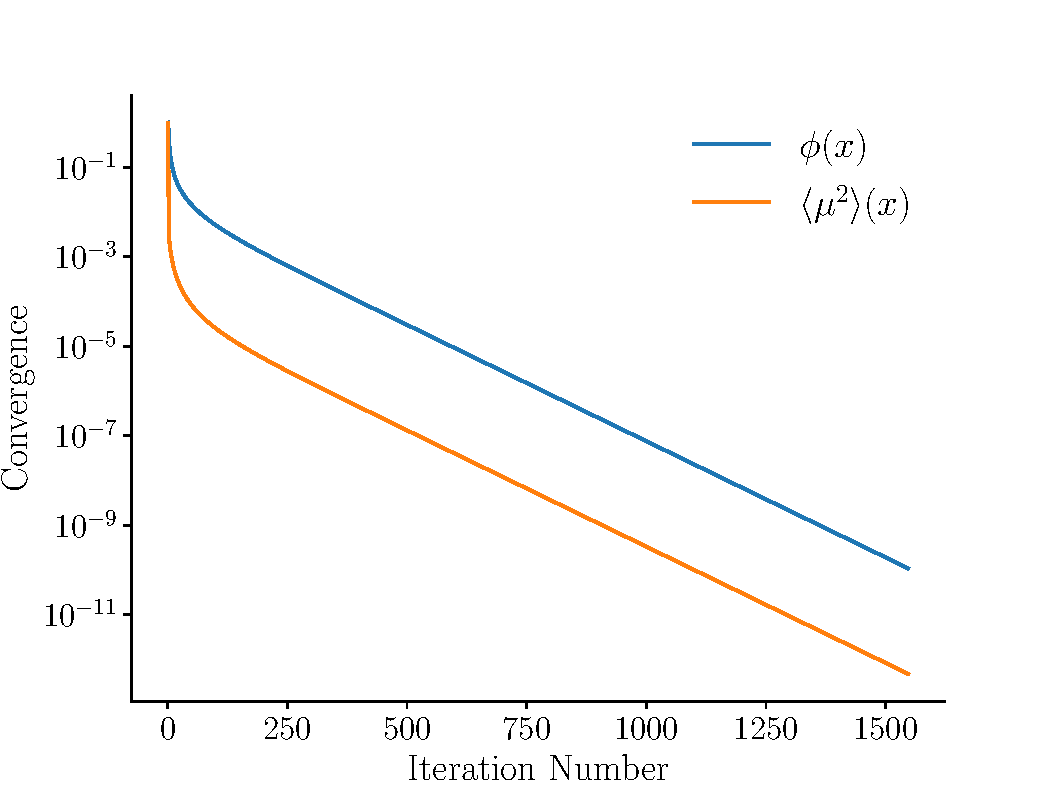
\includegraphics[width=\textwidth]{figs/converge.pdf}
	\caption{}
	\label{fig:si}
\end{subfigure}
\hspace{-2em}
\begin{subfigure}{.515\textwidth}
	\centering
	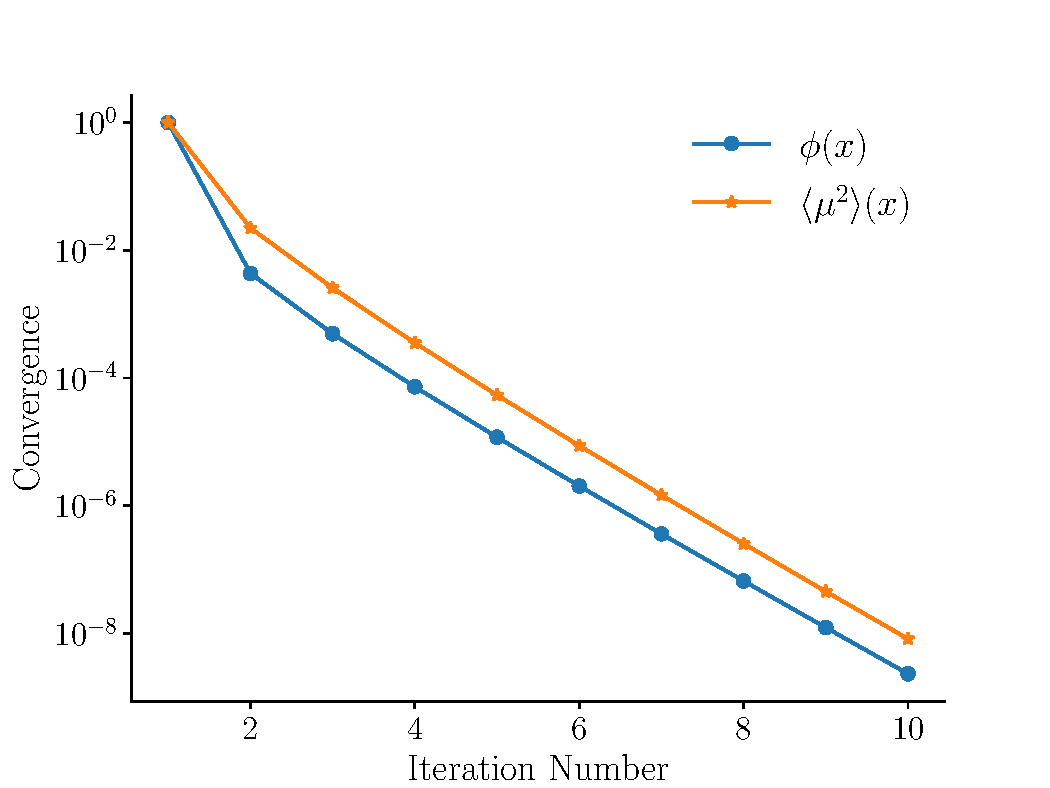
\includegraphics[width=\textwidth]{figs/converge1.pdf}  
	\caption{}
	\label{fig:vef}
\end{subfigure}
\caption{Relative iterative change for $\phi(x)$ and $\edd(x)$ for (a) unaccelerated and (b) VEF accelerated SI. }
\end{figure}

The relative iterative change, defined as 
	\begin{equation}
		\frac{\| f\relll - f\rell \|_2}{\| f\relll \|_2 } \,,
	\end{equation}	
is given in Figure~\ref{fig:si} as a function of unaccelerated iteration number for $f = \phi(x)$ and $f = \edd(x)$. The relative iterative change is a crude measure of iterative convergence.  The Eddington factor's large drop in relative 
iterative change between the first and second iterations supports the claim that the angular shape of the angular flux, and thus the Eddington factor, converges rapidly. When compared to Fig.~\ref{fig:vef}, a plot of the relative iterative change for the VEF method, it is clear that the VEF method transfers the fast rate of convergence of the Eddington factor to the scalar flux. 

	% \begin{figure}
	% 	\centering
	% 	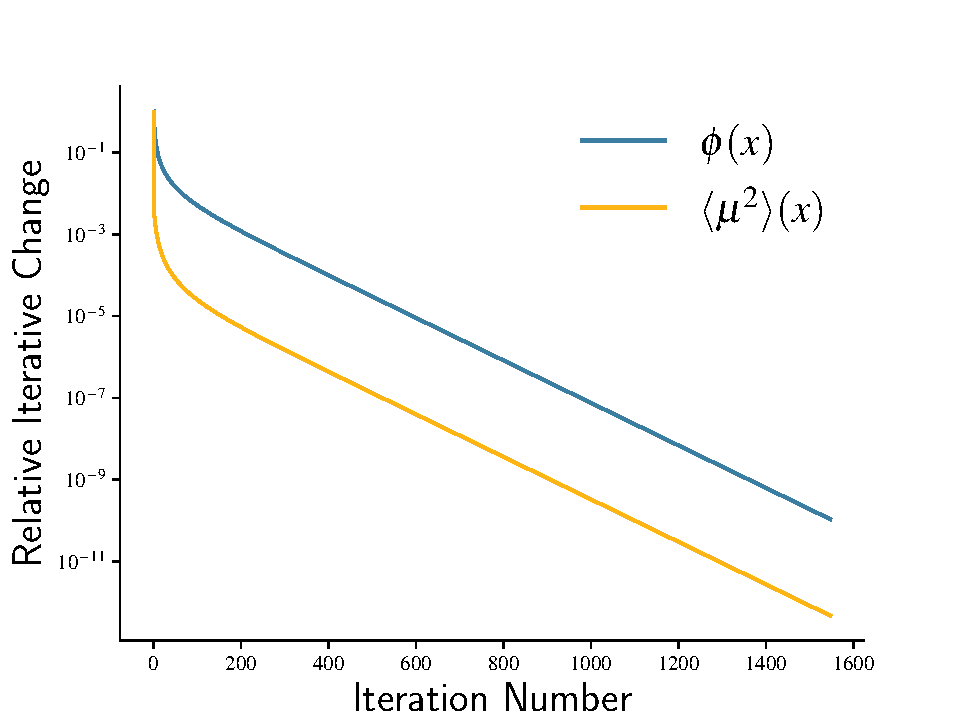
\includegraphics[width=.75\textwidth]{figs/si.pdf}
	% 	\caption{The convergence rate for $\phi(x)$ and $\edd(x)$ for unaccelerated S$_8$ Source Iteration. }
	% 	\label{fig:si}
	% \end{figure}

	% \begin{figure}
	% 	\centering
	% 	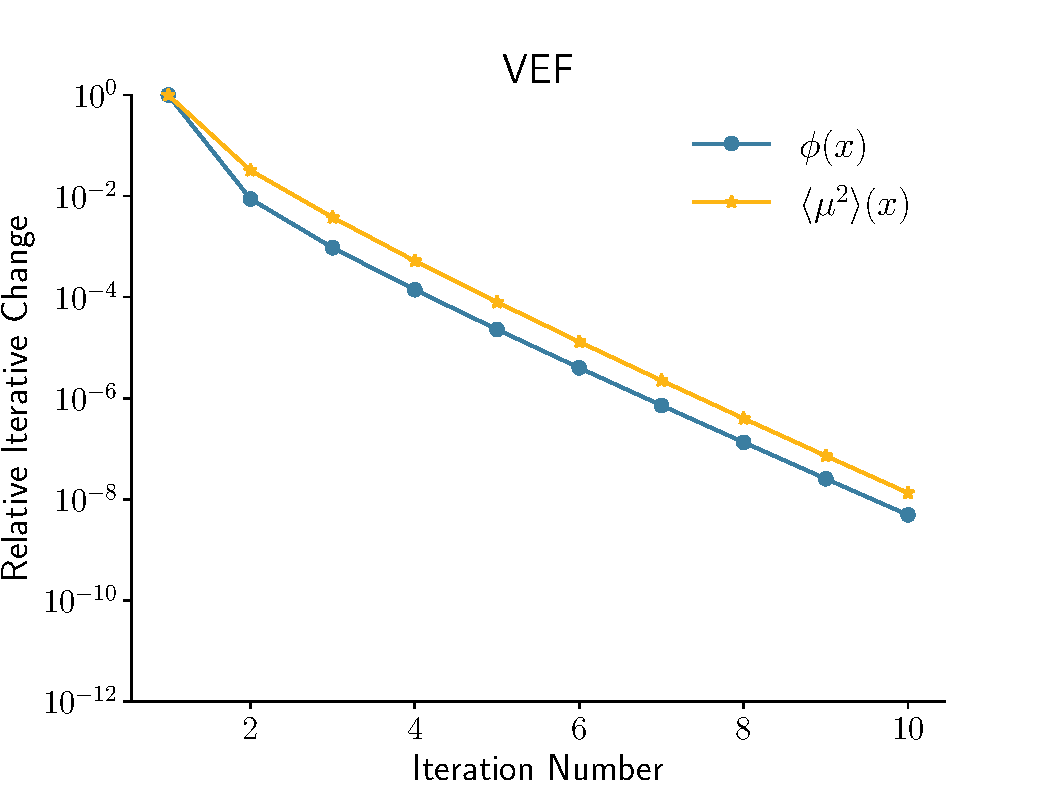
\includegraphics[width=.75\textwidth]{figs/vef.pdf} 
	% 	\caption{The convergence rate for $\phi(x)$ and $\edd(x)$ for VEF accelerated S$_8$. }
	% 	\label{fig:vef}
	% \end{figure}

For the previously-described homogeneous problem, the number of iterations required for convergence of unaccelerated SI, the VEF method, and consistently-differenced S$_2SA$ is plotted in Figure~\ref{fig:si_vef_s2sa} for a range of scattering ratios. The ratio of unaccelerated to VEF accelerated iterations ranged from 1.6 to 267.  As expected, the effectiveness of acceleration for the VEF and S$_2$SA methods is essentially the same. 

	\begin{figure}[htb]
		\centering
		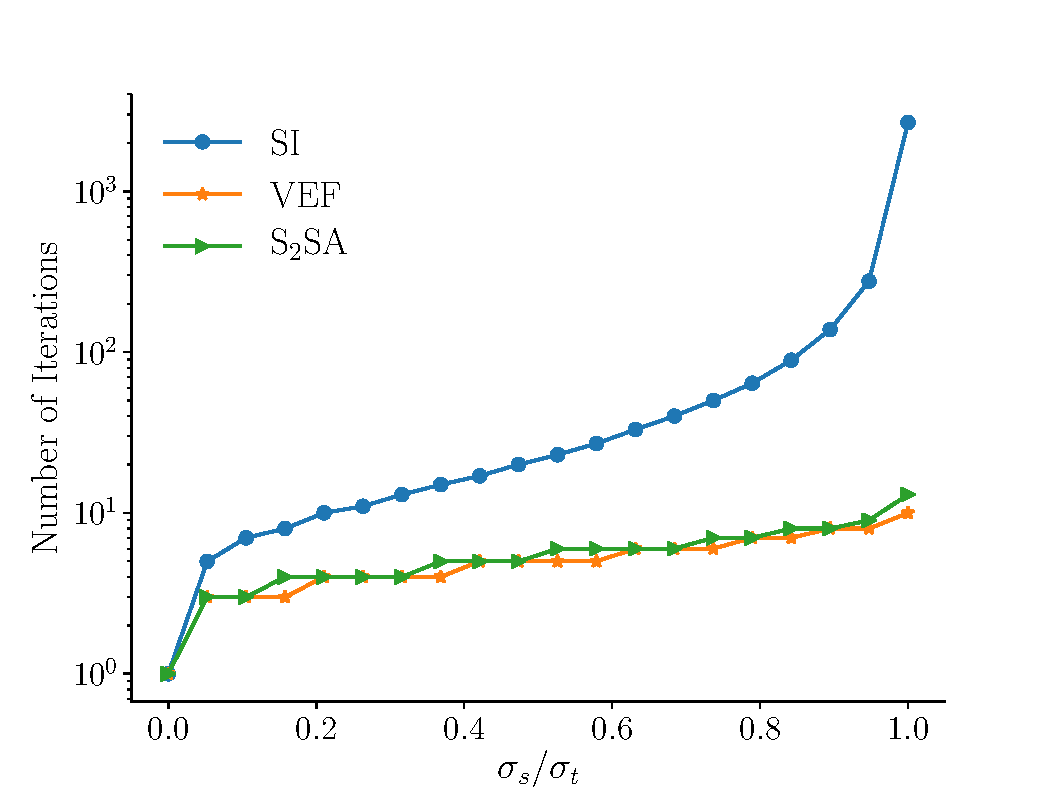
\includegraphics[width=.75\textwidth]{figs/acceleration.pdf} 
		\caption{A comparison of the number of iterations required to converge for Source Iteration, VEF acceleration, and S$_2$SA for varying ratios of $\sigma_s$ to $\sigma_t$. } 
		\label{fig:si_vef_s2sa}
	\end{figure}

The Method of Manufactured Solutions (MMS) was used to compare the spatial accuracy of our VEF method as the cell width was decreased. A solution to Eq. \ref{eq:sn} was assumed as follows: 
		\begin{equation} \label{res:solMMS}
			% \psi_{n,\text{MMS}}(x) = \sin\paren{\frac{\pi x}{x_b}} \,, \quad x\in [0,x_b],
			\psi_{n,\text{MMS}}(x) = \sin\paren{\frac{\pi x}{x_b}} \paren{1 + \mu_n \frac{2x - x_b}{x_b}} \,, \quad x\in[0,x_b] \,, 
		\end{equation}
with the corresponding scalar flux given by
		\begin{equation}
			\phi_\text{MMS}(x) = \sum_{n=1}^N \psi_{n,\text{MMS}}(x) w_n = 2 \sin\paren{\frac{\pi x}{x_b}} \,.
		\end{equation}
Note that this solution satisfies vacuum boundary conditions at $x=0$ and $x=x_b$.
Substituting this solution into the following version of Eq. \ref{eq:sn} with a more general source,
	\begin{equation} \label{eq:snaq}
		\mu_n \dderiv{\psi_n}{x}(x) + \sigma_t(x) \psi_n(x) = 
		\frac{\sigma_s(x)}{2} \phi(x) +  Q_n(x) \,, \quad 1 \leq n \leq N \,,
	\end{equation}\
and solving for $Q_n(x)$ yields:
	\begin{multline} \label{res:fixedSource}
		% Q_{n,\text{MMS}}(x) = \mu_n \frac{\pi}{x_b} \cos\paren{\frac{\pi x}{x_b}} + \bracket{\sigma_t(x) - 
		% \sigma_s(x)}\sin\paren{\frac{\pi x}{x_b}} \,.
		Q_{n,\text{MMS}}(x) = 
			\mu_n\bracket{2\frac{\mu_n}{x_b}\sin\paren{\frac{\pi x}{x_b}} + 
				\frac{\pi}{x_b}\cos\paren{\frac{\pi x}{x_b}}\paren{1 + \mu_n \frac{2x-x_b}{x_b}}}
				\\+ \sigma_t(x)\sin\paren{\frac{\pi x}{x_b}}\paren{1 + \mu_n \frac{2x - x_b}{x_b}} - \sigma_s(x) \sin\paren{\frac{\pi x}{x_b}} \,.
	\end{multline}
Using Eq.~\ref{res:fixedSource} as the fixed source in Eq.~\ref{eq:snaq}, and imposing 
vacuum boundary conditions at $x=0$ and $x=x_b$ makes Eq.~\ref{res:solMMS} the 
analytic solution of Eq. \ref{eq:snaq}.  Thus the difference between a numerical 
solution of Eq.~\ref{eq:snaq} (defined in this way) and the MMS solution is the spatial truncation error of the numerical solution.  
Calculations were performed for the MMS problem using the cross sections of the homogeneous 
problem, but with vacumm conditions at both boundaries and a slab width of \SI{1}{cm}.
The L2 norm of the difference between the numerical and MMS solutions was computed for five logarithmically spaced cell widths between \SI{0.5}{mm} and \SI{0.01}{mm}.  A fit of the following form to the numerical error, $E$,  
\begin{equation}
		E = C h^n
	\end{equation}
was used to determine the order of accuracy, $n$, and the constant of proportionality, $C$. These values are provided in Table \ref{tab:mms} for the VEF method with the flat and van Leer slope reconstruction scattering source update methods. 
 The lower $C$ value for VEF with van Leer reconstructed slopes indicates that constructing a linear scalar flux dependence from the MFEM drift-diffusion flux increases numerical accuracy. Both methods show second-order accuracy as expected from the orders of accuracy of the LLDG and constant-linear MFEM discretizations in isolation. This indicates that while slope reconstruction can affect numerical 
 accuracy it does not affect the order of accuracy of the method. 
	\begin{table}[htb]
	\centering
	\begin{tabular}{|c|c|c|c|}
	\hline
	\hline
	Update Method & Order & $C$ & $R^2$ \\ 
	\hline
		Flat & \num{1.979} & \num{1.18} & \num{9.9999e-01} \\
Linear & \num{1.988} & \num{0.786} & \num{9.9887e-01} \\

	\hline
	\hline
	\end{tabular}
	\caption{The order of accuracy, error, and $R^2$ values for flat and van Leer slope reconstruction scattering source update methods. }
	\label{tab:mms}
	\end{table}
The difference between the \SN solution and the drift-diffusion solution was compared as a function of cell width for the homogeneous slab problem and for a 
modified Reed's problem \cite{reed}. S$_2$SA was used to generate the \SN solution to which the VEF method was compared. In both cases, the left boundary was reflecting and the right boundary was vacuum. The homogeneous slab had a scattering ratio of 0.99. The cross sections and sources for Reed's problem are provided in Table \ref{tab:reedXS}. The L2 norm of the difference between the SI solution and VEF solution is plotted for the flat and van Leer scattering source update methods in Figs.~\ref{fig:homo} and \ref{fig:reed} for the homogeneous slab problem and Reed's problem. 

	\begin{table}[htb]
	 \centering
		\begin{tabular}{|c|c|c|c|c|c|}
			\hline
			& Region 1 & Region 2 & Region 3 & Region 4 & Region 5 \\ 
			\hline 
			$Q$ & 10 & 0 & 0 & 0 & 1 \\ 
			$\sigma_t$ & 10 & 0.001 & 1 & 5 & 1 \\ 
			$\sigma_a$ & 10 & 0 & 0.1 & 0 & 0.1 \\ 
			\hline 
			Domain & $0 \leq x < 2$ & $2 \leq x < 4$ & $4\leq x < 6$ &
				$6 \leq x < 7$ & $7 \leq x \leq 8$\\ 
			\hline 
		\end{tabular}
		\caption{The cross sections and source used for Reed's problem.}
		\label{tab:reedXS}
	\end{table}

	\begin{figure}[htb]
		\centering
		\begin{subfigure}{.5\textwidth}
			\centering
			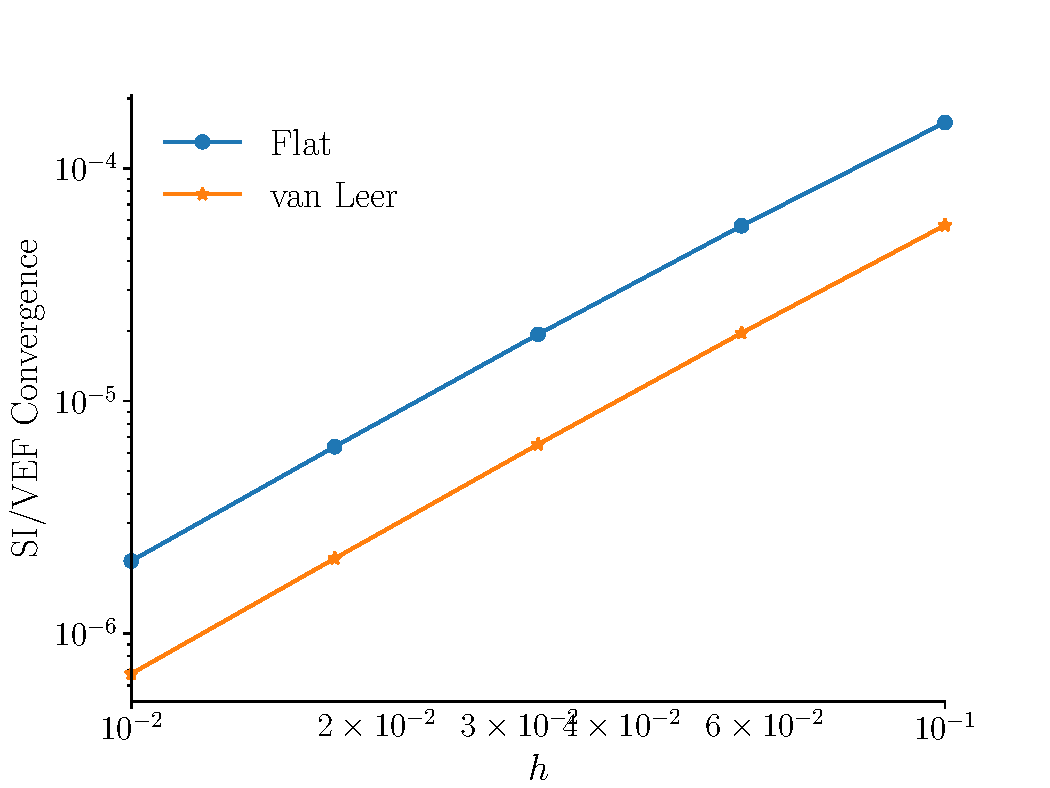
\includegraphics[width=\textwidth]{figs/solconv.pdf}
			\caption{}
			\label{fig:homo}
		\end{subfigure}
		\hspace{-2em}
		\begin{subfigure}{.5\textwidth}
			\centering
			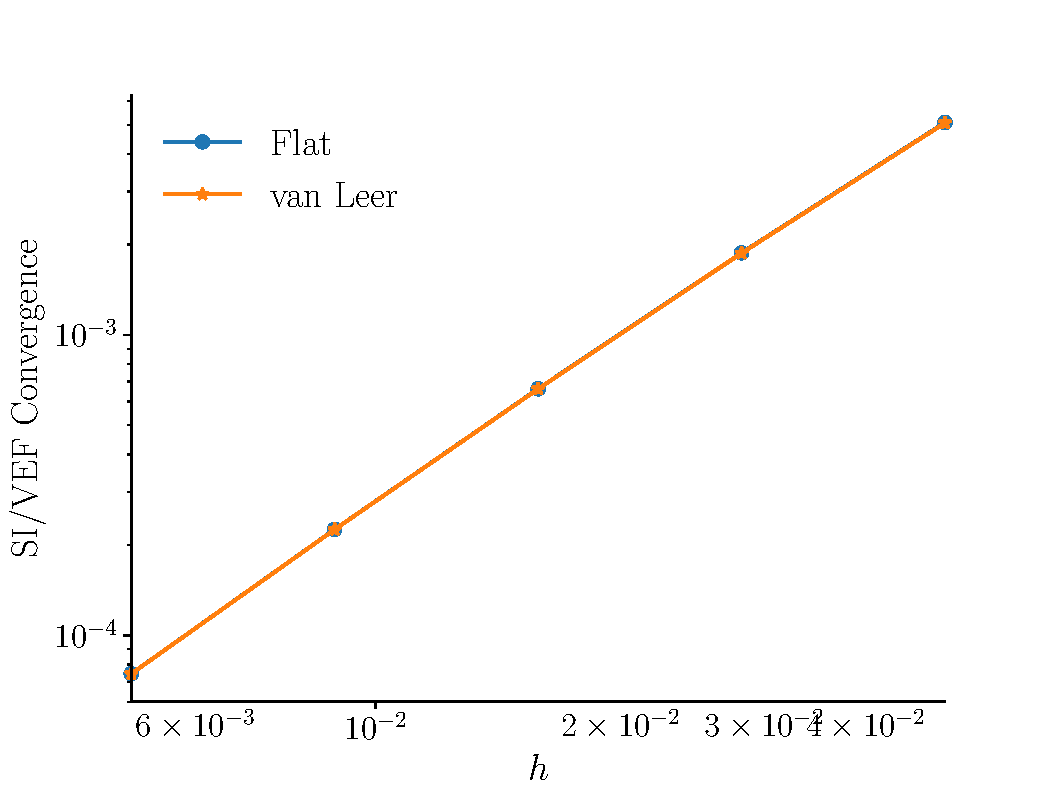
\includegraphics[width=\textwidth]{figs/solconv1.pdf}
			\caption{}
			\label{fig:reed}
		\end{subfigure}
		\caption{The L2 norm of the difference between the \SN and drift-diffusion solutions as a function of cell width for the two scattering source update methods. Results for the homogeneous problem and Reed's problem are given in (a) and (b), respectively.}
	\end{figure}

In the homogeneous problem, VEF with van Leer limited slope reconstruction was three times closer to the \SN solution than VEF without reconstruction. However, in Reed's problem, reconstruction did not affect the convergence of drift-diffusion to \SN. This could be due to the fact that the flux derivatives are discontinuous at material interfaces and the cell-centered slope reconstruction method has no knowledge of these discontinuities. 

Lastly, the VEF method was tested in the diffusion limit. Calculations were performed for several variants of the homogeneous problem. 
These problems differed from the homogeneous problem only with respect to the cross sections and fixed source, which were scaled as follows \cite{diflim}: 
	\begin{subequations} \label{res:scaling}
		\begin{equation} 
			\sigma_t(x) \rightarrow \sigma_t(x)/\epsilon \,, 
		\end{equation}
		\begin{equation}
			\sigma_a(x) \rightarrow \epsilon \sigma_a(x) \,,
		\end{equation}
		\begin{equation}
			Q(x) \rightarrow \epsilon Q(x) \,, 
		\end{equation}
	\end{subequations}
with $\sigma_t=\sigma_a=$ \SI{1}{cm^{-1}} and $Q = \SI{1}{\particles\per\second\per\cm\cubed}$.  As $\epsilon \rightarrow 0$, the system becomes diffusive. The number of iterations until convergence as $\epsilon \rightarrow 0$ is provided in Table \ref{tab:diffLim}. 
% The error between the VEF solution and the exact diffusion solution is provided in Fig.~\ref{fig:dl_err}. 
These results support the claim that the VEF method is robust in the diffusion limit as both scattering update methods properly preserved the thick diffusion limit. 
	\begin{table}[htb]
	\centering
	\begin{tabular}{|c|c|c|c|}
	\hline
	\hline
	$\epsilon$ & Flat & Linear \\ 
	\hline
		\num{1.0e-01} & 6 & 6 \\
\num{1.0e-02} & 3 & 3 \\
\num{1.0e-03} & 2 & 2 \\
\num{1.0e-04} & 2 & 2 \\
\num{1.0e-05} & 2 & 2 \\

	\hline
	\hline
	\end{tabular}
	\caption{The number of iterations until convergence for a range of $\epsilon$ values for the flat and linear scattering update methods. }
	\label{tab:diffLim}
	\end{table}
	
	% \begin{figure}[htb]
	% 	\centering
	% 	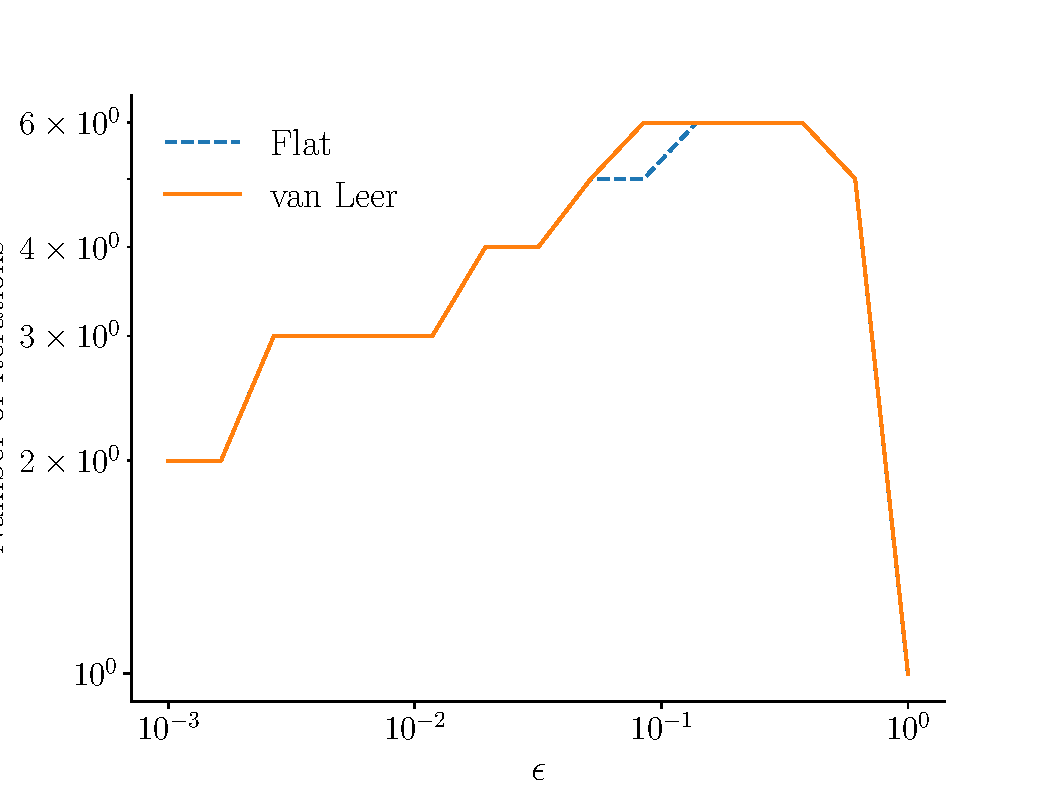
\includegraphics[width=.75\textwidth]{figs/perm_dl.pdf}
	% 	\caption{The number of iterations required for convergence in the diffusion limit ($\epsilon \rightarrow 0$). }
	% 	\label{fig:dl_it}
	% \end{figure}
	% \begin{figure}
	% 	\centering
	% 	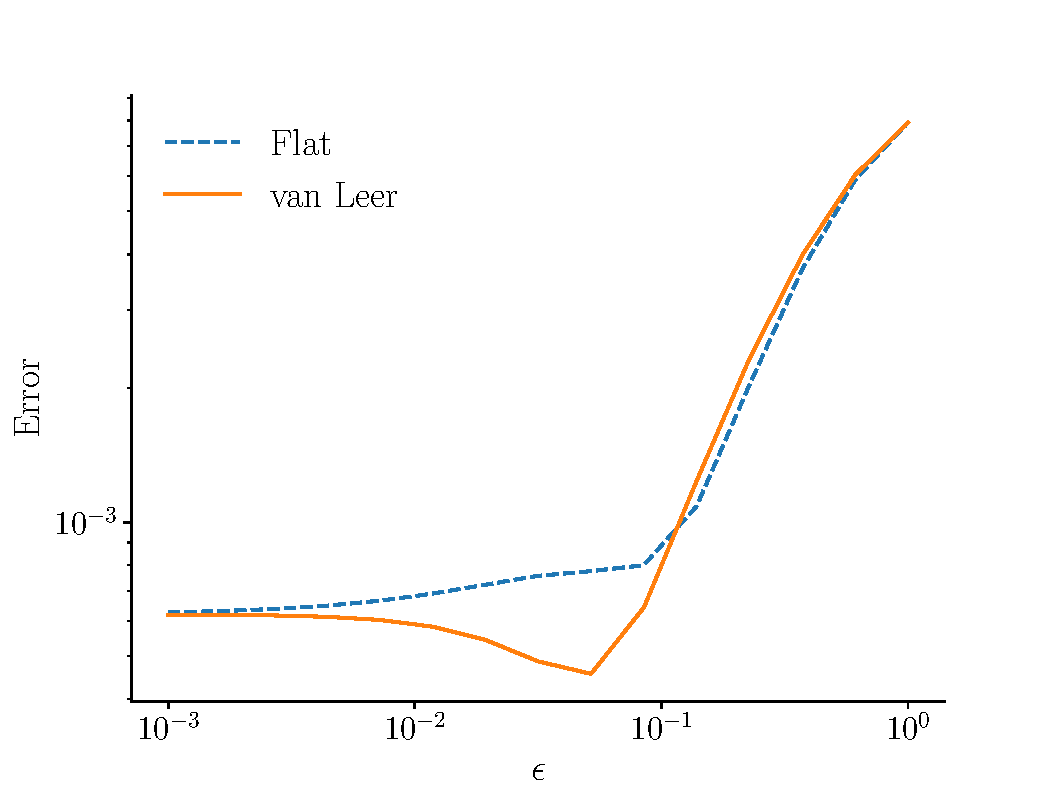
\includegraphics[width=.75\textwidth]{figs/perm_dl1.pdf}
	% 	\caption{The error between the VEF methods and the exact diffusion solution as $\epsilon \rightarrow 0$. }
	% 	\label{fig:dl_err}
	% \end{figure}
	% \begin{figure}
	% 	\centering
	% 	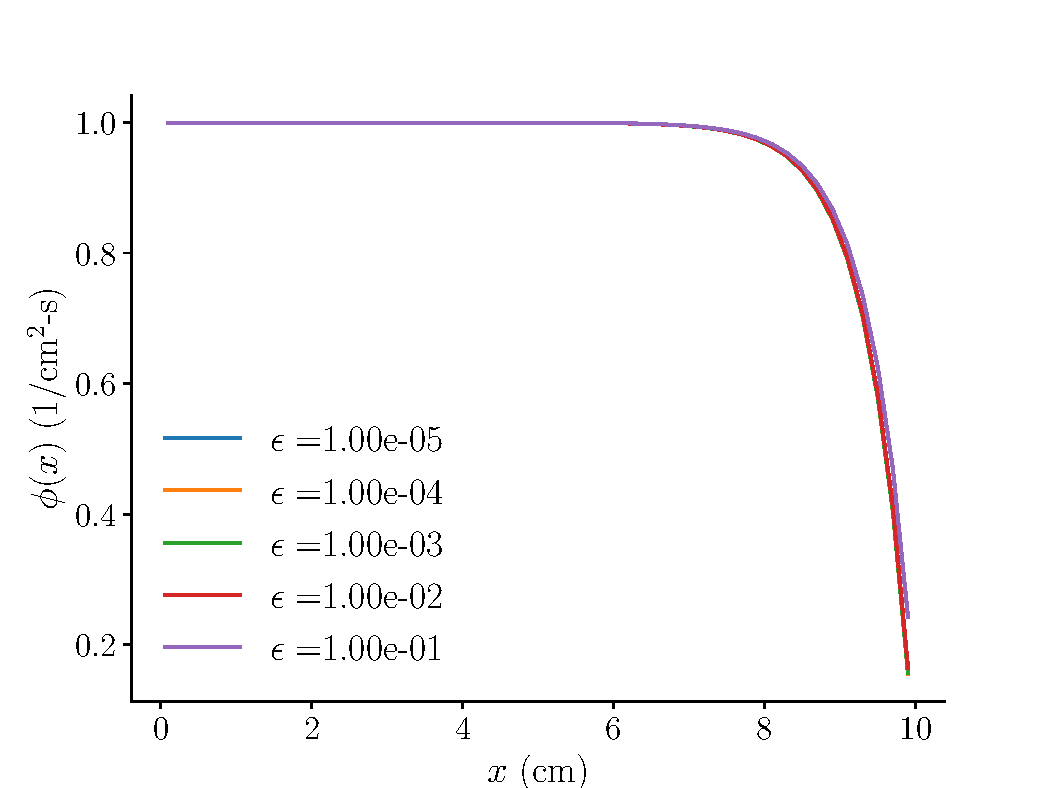
\includegraphics[width=.75\textwidth]{figs/profile.pdf}
	% 	\caption{The scalar flux profiles }
	% 	\label{fig:flux_profiles}
	% \end{figure}